\section{Phân tích khám phá dữ liệu (EDA)}
\label{sec:eda}

Phần này trình bày kết quả phân tích khám phá dữ liệu\cite{tukey1977eda} trên cả hai nguồn. Các phân tích bao gồm thống kê mô tả, phân phối biến mục tiêu, phân tích đơn biến (univariate) và đa biến (multivariate), cùng kiểm tra tương quan giữa các thuộc tính.

\subsection{Thống kê mô tả tổng quan}

\cref{tab:descriptive-chotot} tóm tắt thống kê mô tả các biến numeric chính của Chợ Tốt.

\begin{table}[H]
    \centering
    \caption{Thống kê mô tả --- Chợ Tốt (biến numeric sau cleaning)}
    \label{tab:descriptive-chotot}
    \begin{tabular}{lrrrrr}
        \toprule
        \textbf{Biến} & \textbf{N} & \textbf{Mean} & \textbf{Median} & \textbf{IQR} & \textbf{Missing (\%)} \\
        \midrule
        price (triệu VND)     & 5.865 & 12.5 & 8.0 & 5.0--15.0 & 0.02 \\
        RAM (GB)               & 5.627 & 10.1 & 8.0 & 8--16 & 4.1 \\
        Storage (GB)           & 5.396 & 373  & 256 & 256--512 & 8.0 \\
        Kích cỡ màn hình (inch) & 4.810 & 14.5 & 14.0 & 13--15.6 & 18.0 \\
        \bottomrule
    \end{tabular}
\end{table}

\begin{table}[H]
    \centering
    \caption{Thống kê mô tả --- Websosanh (biến numeric sau cleaning)}
    \label{tab:descriptive-websach}
    \begin{tabular}{lrrrrr}
        \toprule
        \textbf{Biến} & \textbf{N} & \textbf{Mean} & \textbf{Median} & \textbf{IQR} & \textbf{Missing (\%)} \\
        \midrule
        price\_median (triệu VND) & 4.384 & 23.6 & 18.0 & 12.5--29.0 & 0 \\
        RAM (GB)                   & 4.361 & 14.2 & 16.0 & 8--16 & 0.5 \\
        Storage (GB)               & 4.159 & 584  & 512 & 512--1024 & 5.1 \\
        Kích thước (inch)          & 4.288 & 14.8 & 15.3 & 14--15.6 & 2.2 \\
        \bottomrule
    \end{tabular}
\end{table}

Sự chênh lệch median giá giữa hai nguồn (8 triệu vs 18 triệu) phản ánh đúng bản chất: Chợ Tốt là laptop second-hand, Websosanh là laptop mới.

\subsection{Phân phối biến mục tiêu (Label Distribution)}
\label{subsec:label-distribution}

\subsubsection{Chợ Tốt}
Giá đăng bán có phân phối lệch phải (right-skewed) với mean $\approx$ 12.5 triệu và median $\approx$ 8 triệu VND. Nhóm giá dưới 15 triệu chiếm đa số; nhóm high-end ($>$ 50 triệu) chỉ chiếm $\sim$3\% nhưng kéo đuôi phải đáng kể.

\begin{figure}[H]
    \centering
    % FILL-IN: [USER] Thêm biểu đồ phân phối giá Chợ Tốt
    % Nguồn: notebook 01a, cell [33] — histogram + KDE + boxplot giá
    % \includegraphics[width=0.8\textwidth]{images/price-dist-chotot.png}
    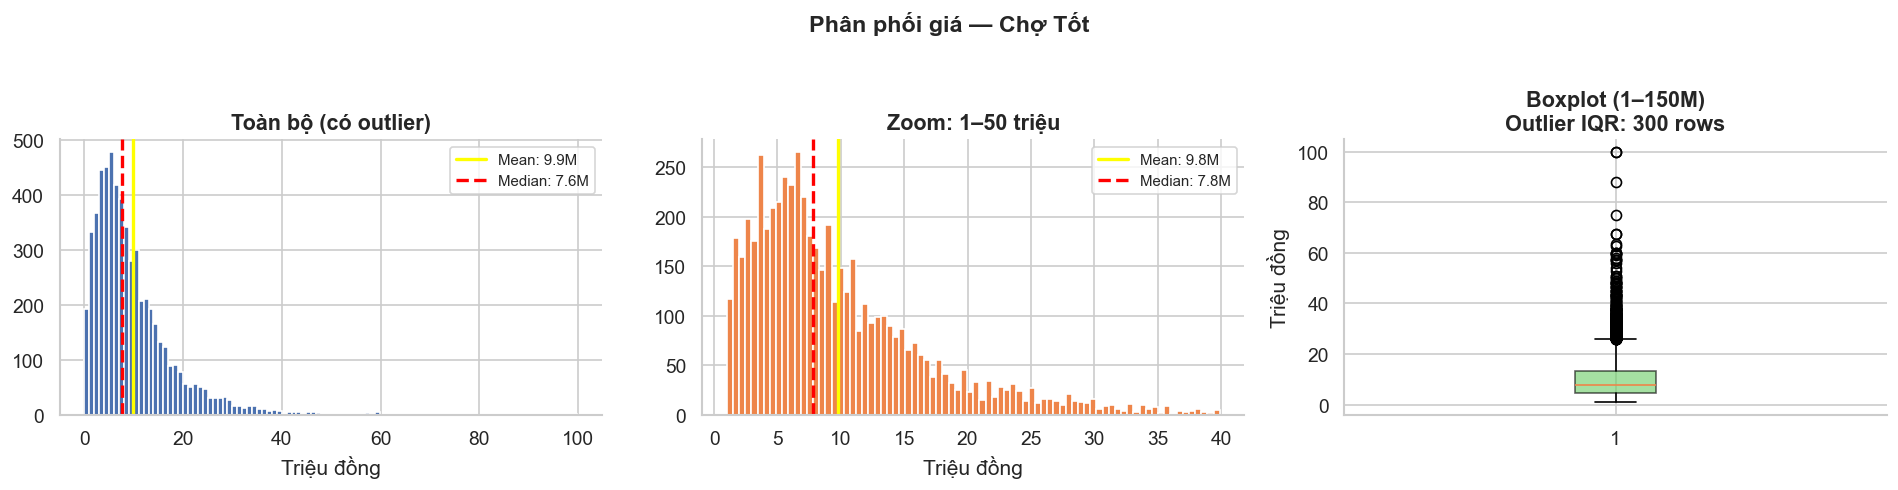
\includegraphics[width=0.8\textwidth]{images/chotot_img_06.png}
    \caption{Phân phối giá laptop trên Chợ Tốt. Histogram (trái) và boxplot (phải) cho thấy dữ liệu lệch phải rõ rệt, với median thấp hơn mean --- đặc trưng của right-skewed distribution.}
    \label{fig:price-dist-chotot}
\end{figure}

\subsubsection{Websosanh}
Biến \texttt{price\_median} (tính từ median 3 nguồn giá) cũng lệch phải nhưng ít hơn so với Chợ Tốt. Skewness $\approx$ 2.65, range từ 3 triệu đến 179.4 triệu VND. Log-transform giúp chuẩn hóa phân phối đáng kể.

\begin{figure}[H]
    \centering
    % FILL-IN: [USER] Thêm biểu đồ phân phối giá Websosanh (gốc vs log)
    % Nguồn: notebook 01b — histogram price_median vs log_price_median
    % \includegraphics[width=0.8\textwidth]{images/price-dist-websach.png}
    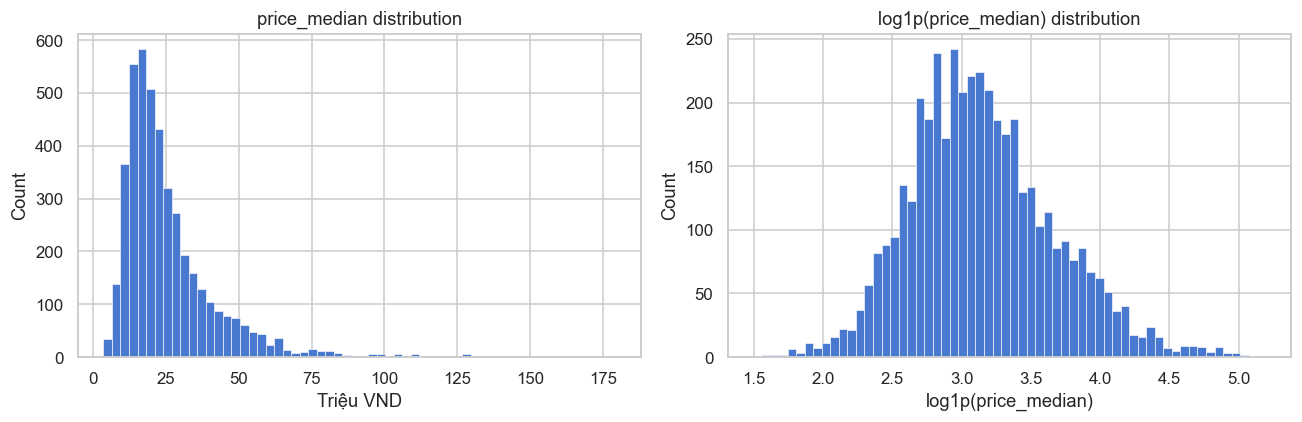
\includegraphics[width=0.8\textwidth]{images/websach_img_20.png}
    \caption{Phân phối giá Websosanh trước và sau log-transform. Log-transform giảm skewness, giúp phân phối gần chuẩn hơn.}
    \label{fig:price-dist-websach}
\end{figure}

\subsection{Phân tích đơn biến}
\label{subsec:univariate}

\subsubsection{Phân phối Brand}

Cả hai nguồn đều cho thấy sự tập trung vào 5 hãng chính: Dell, HP, Asus, Lenovo, và Apple. Trên Chợ Tốt, 5 hãng này chiếm $\sim$80\% listing. Các hãng hiếm ($<$ 30 listing) bao gồm Sony, Fujitsu, Toshiba được cân nhắc gom vào nhóm ``Khác'' khi modeling.

\begin{figure}[H]
    \centering
    % FILL-IN: [USER] Thêm biểu đồ phân phối brand
    % Nguồn: notebook 01a, cell [76] — bar chart brand distribution
    % \includegraphics[width=0.7\textwidth]{images/brand-distribution.png}
    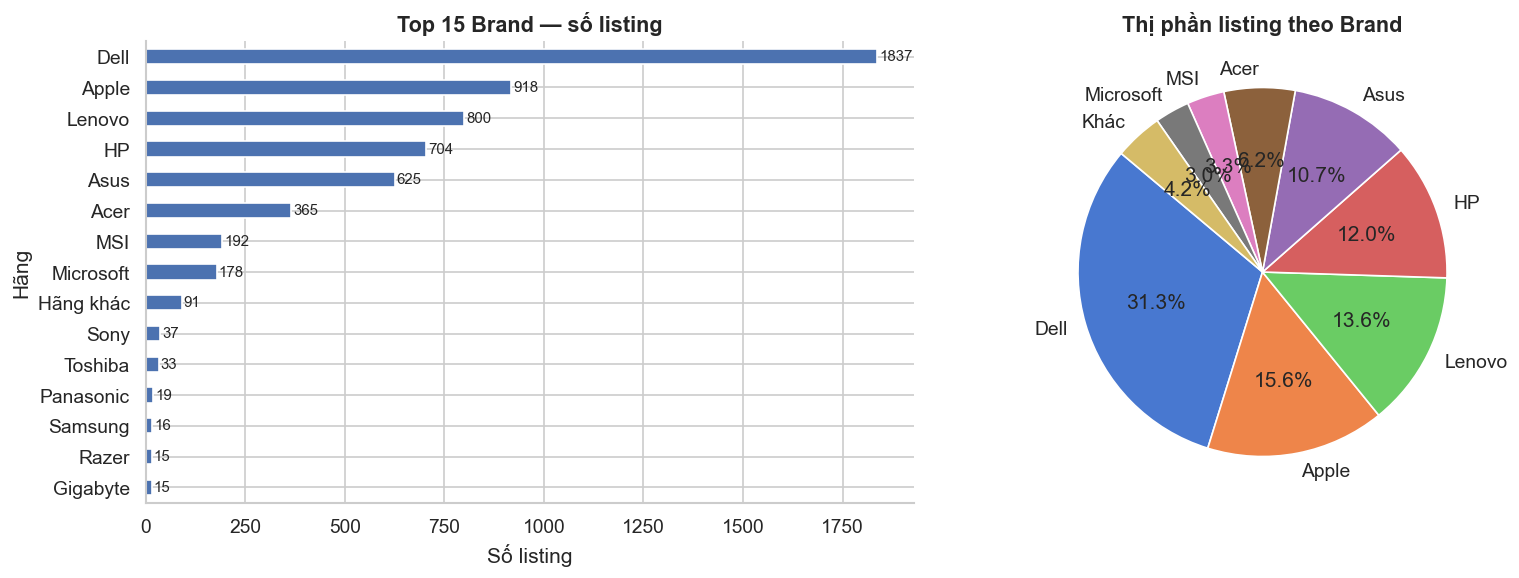
\includegraphics[width=0.7\textwidth]{images/chotot_img_14.png}
    \caption{Phân phối số lượng listing theo brand trên Chợ Tốt. Dell và HP dẫn đầu, theo sau là Asus, Lenovo và Apple.}
    \label{fig:brand-distribution}
\end{figure}

\subsubsection{CPU Brand và CPU Tier}

Intel chiếm $\sim$79.5\% (Chợ Tốt) và $\sim$80.8\% (Websosanh). AMD chiếm 13--15\%, Apple $\sim$3\%, Qualcomm và Microsoft SQ dưới 1\%.

Phân loại CPU tier cho thấy tín hiệu giá rõ: median giá tăng theo thứ tự i3/Ryzen 3 $<$ i5/Ryzen 5 $<$ i7/Ryzen 7 $<$ i9/Ryzen 9. Tuy nhiên CPU tier có confounding với RAM, GPU, và brand (laptop high-end thường có CPU, RAM, GPU đều cao).

\begin{figure}[H]
    \centering
    % FILL-IN: [USER] Thêm biểu đồ CPU distribution + price by CPU tier
    % Nguồn: notebook 01a, cell [170] — subplots CPU brand + CPU tier
    % \includegraphics[width=0.85\textwidth]{images/cpu-analysis.png}
    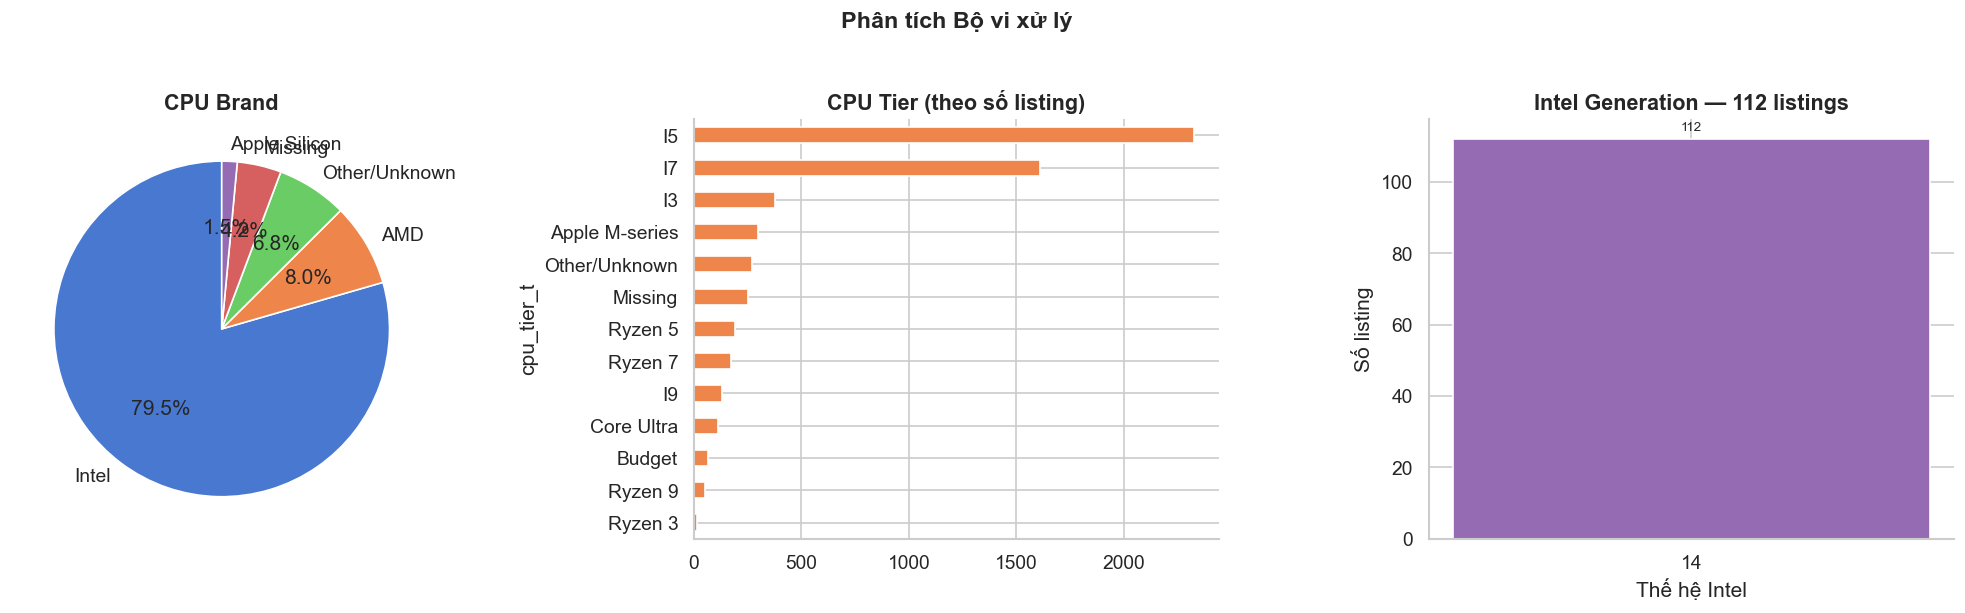
\includegraphics[width=0.85\textwidth]{images/chotot_img_27.png}
    \caption{Phân phối CPU brand (trái) và phân phối giá theo CPU tier (phải). Intel chiếm đa số, giá tăng rõ theo tier.}
    \label{fig:cpu-analysis}
\end{figure}

\subsubsection{RAM}

Hai mức RAM phổ biến nhất là 8GB ($\sim$43\%) và 16GB ($\sim$39\%), cùng chiếm 82.2\% dữ liệu Chợ Tốt. Giá tăng rõ rệt từ 4GB $\rightarrow$ 8GB $\rightarrow$ 16GB $\rightarrow$ 32GB, nhưng mối quan hệ ở các mức hiếm ($<$ 4GB, $>$ 32GB) không ổn định do ít mẫu.

\begin{figure}[H]
    \centering
    % FILL-IN: [USER] Thêm biểu đồ RAM distribution + price by RAM
    % Nguồn: notebook 01a, cell [190] — bar chart + boxplot
    % \includegraphics[width=0.85\textwidth]{images/ram-analysis.png}
    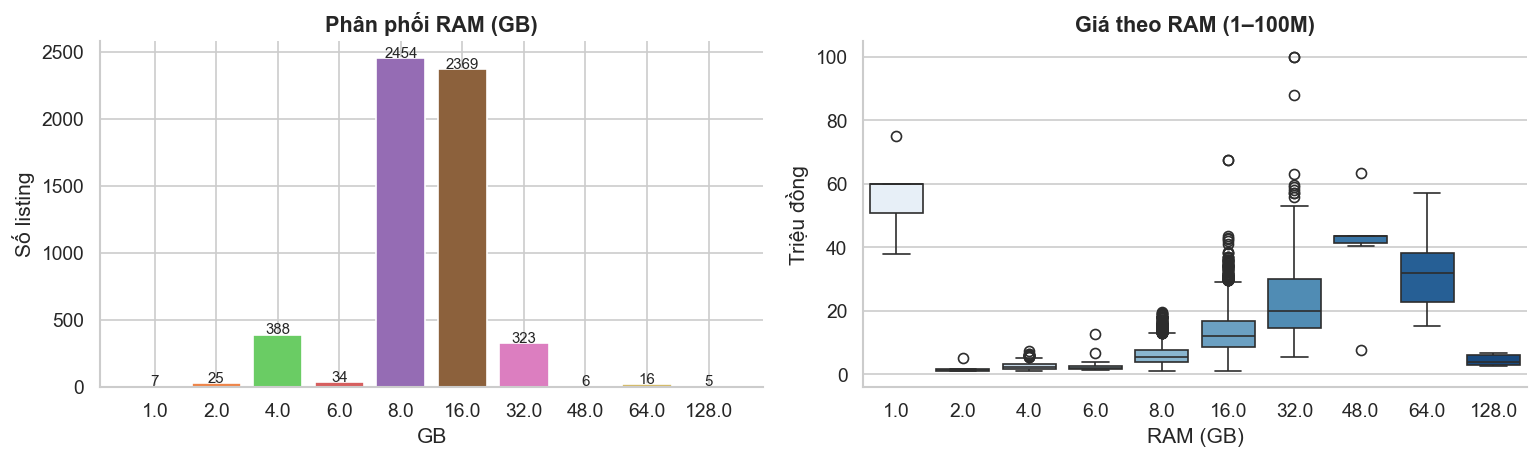
\includegraphics[width=0.85\textwidth]{images/chotot_img_30.png}
    \caption{Phân phối RAM và giá theo mức RAM trên Chợ Tốt. 8GB và 16GB chiếm đa số, giá tăng đơn điệu theo dung lượng ở các mức phổ biến.}
    \label{fig:ram-analysis}
\end{figure}

\subsubsection{GPU}

GPU có tỷ lệ missing cao nhất ($\sim$24\% trên Chợ Tốt, $\sim$4.7\% trên Websosanh). Phân loại GPU tier cho thấy phần lớn là Intel Integrated (UHD/Iris Xe). Nhóm Dedicated GPU (RTX/GTX) có median giá cao hơn đáng kể.

Missing GPU có tính hệ thống theo brand: HP ($\sim$34\% missing) cao hơn Dell ($\sim$19\%).

\subsubsection{Storage}

SSD chiếm ưu thế tuyệt đối ở cả hai nguồn. Dung lượng phổ biến nhất là 256GB và 512GB (Chợ Tốt) hoặc 512GB (Websosanh). Giá tăng theo storage tier: 256GB $<$ 512GB $<$ 1TB $<$ 2TB, tuy nhiên hiệu ứng bị confounding bởi các yếu tố khác.

\subsubsection{Kích thước màn hình}

Nhóm 14--14.9 inch phổ biến nhất ở cả hai nguồn. Giá có xu hướng tăng ở nhóm $\geq$16 inch, nhưng hiệu ứng bị nhiễu bởi cấu hình đi kèm (laptop 16 inch thường là gaming/workstation với GPU rời).

Trên Websosanh, gom kích thước thành 6 nhóm: $<$13, 13--13.9, 14--14.9, 15--15.9, 16--16.9, và $\geq$17 inch.

\subsection{Phân tích đa biến}
\label{subsec:multivariate}

\subsubsection{Giá theo Brand}

Boxplot giá theo top-10 brand cho thấy Apple có median giá cao nhất và IQR rộng nhất. Dell, HP, Lenovo tập trung ở phân khúc trung bình. MSI (gaming) có median cao thứ 2.

\begin{figure}[H]
    \centering
    % FILL-IN: [USER] Thêm boxplot giá theo brand
    % Nguồn: notebook 01a, cell [37] — boxplot price by top-10 brands
    % \includegraphics[width=0.8\textwidth]{images/price-by-brand.png}
    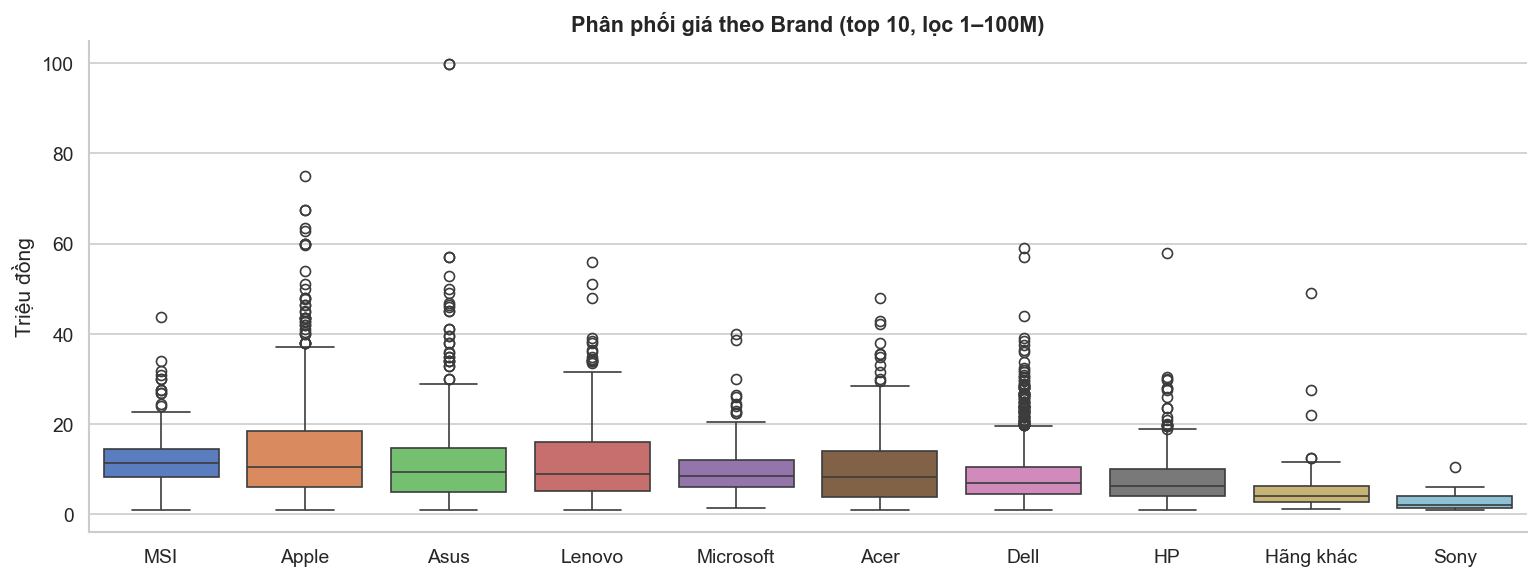
\includegraphics[width=0.8\textwidth]{images/chotot_img_07.png}
    \caption{Phân phối giá theo brand (top 10) trên Chợ Tốt. Apple có median và spread cao nhất, phản ánh định vị premium.}
    \label{fig:price-by-brand}
\end{figure}

\subsubsection{Tương tác giữa các thuộc tính}

Phân tích interaction cho thấy các feature cấu hình không độc lập khi giải thích giá:

\begin{itemize}[noitemsep]
    \item \textbf{CPU $\times$ RAM}: Giá tăng đồng thời theo CPU tier và RAM. Với cùng mức RAM, laptop Intel i7 có giá cao hơn i5; với cùng CPU, RAM 16GB có giá cao hơn 8GB.
    \item \textbf{GPU $\times$ RAM}: Median giá tăng mạnh khi RAM cao kết hợp GPU rời, đặc biệt ở nhóm RTX. Tổ hợp RAM $\geq$16GB + RTX có giá gấp 2--3 lần so với 8GB + Intel Integrated.
    \item \textbf{RAM $\times$ Storage}: Giá tăng rõ khi cả RAM tier và storage tier cùng tăng. Tổ hợp 32GB + 2TB có median price rất cao.
    \item \textbf{Brand $\times$ Screen size}: Cùng nhóm 16--16.9 inch, Apple và MSI có median cao hơn nhiều so với HP hoặc Lenovo.
\end{itemize}

Các tương tác này cho thấy mô hình tuyến tính cần interaction features, hoặc ưu tiên sử dụng tree-based models có thể tự học tương tác phi tuyến\cite{breiman2001random}.

\begin{figure}[H]
    \centering
    % FILL-IN: [USER] Thêm heatmap RAM × Brand × Price
    % Nguồn: notebook 01a, cell [202] — heatmap median price by brand and RAM
    % \includegraphics[width=0.7\textwidth]{images/ram-brand-heatmap.png}
    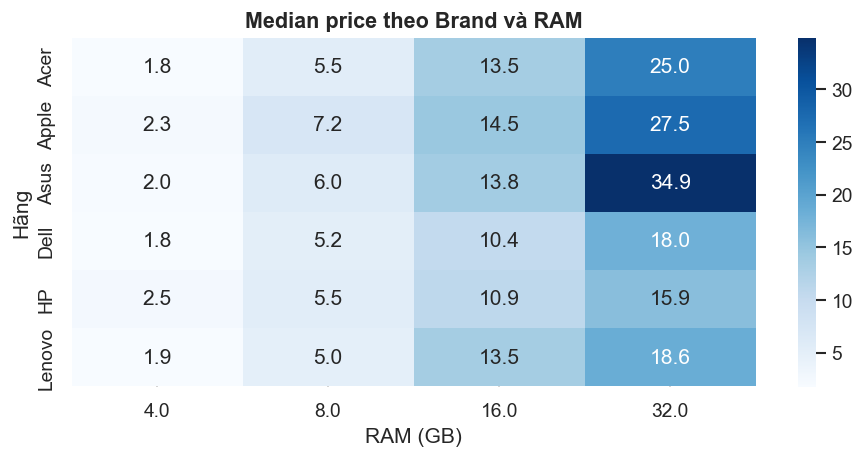
\includegraphics[width=0.7\textwidth]{images/chotot_img_33.png}
    \caption{Heatmap median giá (triệu VND) theo brand và mức RAM trên Chợ Tốt. Giá tăng theo cả hai chiều, với Apple/MSI ở mức cao nhất.}
    \label{fig:ram-brand-heatmap}
\end{figure}

\subsubsection{Tương quan (Correlation)}

Trên Chợ Tốt, RAM có tương quan dương vừa phải với log(price) ($r \approx 0.53$). Storage cũng có tương quan dương nhưng yếu hơn. Tương quan giữa RAM và storage ($r \approx 0.35$) cho thấy multicollinearity ở mức chấp nhận được.

\subsubsection{Phân phối Tình trạng (riêng Chợ Tốt)}

Nhóm ``đã sử dụng chưa sửa'' chiếm $\sim$95\%, gây class imbalance nghiêm trọng. Phát hiện $\sim$90 dòng gắn nhãn ``Mới'' nhưng title chứa keyword second-hand (``đẹp 98\%'', ``pin'', ``góp''), cho thấy label noise.

\subsection{Phân tích dữ liệu phi cấu trúc: Title}
\label{subsec:text-analysis}

Cột \texttt{title} trên Chợ Tốt là text tự do do người dùng nhập. Phân tích cho thấy:
\begin{itemize}[noitemsep]
    \item \textbf{Chất lượng tốt}: 100\% không rỗng, 0\% chỉ chứa khoảng trắng.
    \item \textbf{Brand coverage}: $>$90\% title chứa tên brand, xác nhận tính nhất quán với cột \texttt{Hãng}.
    \item \textbf{Spec keywords}: $\sim$55\% chứa thông tin RAM (pattern ``Xgb'', ``X GB''), $\sim$45\% chứa thông tin storage, $\sim$60\% chứa CPU model.
    \item \textbf{Pattern bán cấu trúc}: 585 title chứa pattern ``X/Y'' (ví dụ ``i5/8GB/256GB''), có thể extract spec từ đây.
    \item \textbf{Rủi ro false positive}: Khi extract RAM bằng regex, giá trị storage (``256GB'', ``512GB'') dễ bị nhầm lẫn. Cần rule loại trừ các giá trị $\geq$ 128 khi parse RAM.
\end{itemize}

\subsection{Dòng máy (Model Line) --- riêng Chợ Tốt}

Cột \texttt{Dòng máy} có 458 giá trị unique, phân phối long-tail cực đoan: 88 dòng máy phổ biến nhất cover 80\% dữ liệu, nhưng 370 dòng còn lại chỉ chiếm 20\%. Khoảng 15\% listing gắn nhãn ``Dòng Khác''. Giá có tín hiệu rõ theo dòng máy (ví dụ MacBook Pro $>$ ThinkPad $>$ Inspiron), nhưng IQR rộng ở hầu hết các dòng.

Để giảm high-cardinality, các dòng có $<$ 10 listing được gom vào ``Other''. Kết hợp Hãng + Dòng máy cho tín hiệu giá mạnh hơn dùng riêng lẻ.
